\chapter{Marco teórico}

En esta sección se describirán varios conceptos que serán útiles en el desarrollo de las siguientes secciones.

\section{Reinforcement Learning}

Es un área del aprendizaje automático, que se inspira en la psicología conductista. Básicamente consiste en qué acción debe seleccionar un agente dentro de un entorno para maximizar una recompensa en el largo plazo. El medio ambiente es normalmente modelado como un \ac{MDP}. El planteamiento de un problema en \ac{RL} siempre consta de 3 partes: las sensaciones (que determinan los estados), las acciones, y los objetivos (que determinan las recompensas) \cite{sutton1998reinforcement}.

Los elementos de un \ac{RL} son:
\begin{itemize}
\item \textbf{Estados}, conjunto de características que indican como está el ambiente en cada momento
\item \textbf{Acciones}, acciones disponibles en cada estado que pueden modificar el ambiente
\item \textbf{Política}, mapea estados a acciones
\item \textbf{Función de recompensa}, define el objetivo. Mapea un estado o par de (estado, accion) a una recompensa
\item \textbf{Función de valor}, es un valor numérico que define que tan bueno es un estado o par de (estado, accion) a largo plazo
\end{itemize}

Siempre existe el problema de balancear la exploración con la explotación. Siendo que la explotación nos permite utilizar los conocimientos que ya tenemos para obtener la máxima recompensa, pero la exploración nos permite obtener un mejor conocimiento y así mejorar nuestras decisiones. Si sólo se hiciera exploración, no tendría sentido puesto que nunca se explotaría el conocimiento generado. Y si siempre se hiciera explotación, quedaríamos atorados en la toma de decisiones sub-óptimas. Lo ideal es que haya una alta tasa de exploración al comienzo y que esta vaya disminuyendo hasta un valor pequeño estable con el tiempo.

Los métodos tradicionales de \ac{RL} han utilizado tablas como función de valor para mantener el retorno estimado de cada estado. Ejemplos de tales técnicas son los métodos de Monte Carlo, diferencias temporales y Q-learning. Sin embargo cuando el espacio de estados es demasiado grande, estas técnicas son imposibles de aplicar y se necesita el uso de nuevos métodos que serán descritos en este trabajo.


\subsection{Retorno esperado}

El retorno esperado $G_t$ es la cantidad de recompensa futura que se puede esperar partiendo de un estado, como se puede ver en su fórmula en la ecuación \eqref{eq:retorno_esperado}, donde $R_t$ es la recompensa en el tiempo $t$ y $T$ es el último paso del episodio.

\begin{equation} \label{eq:retorno_esperado}
G_t = R_{t+1} + R_{t+2} + R_{t+3} + ... + R_T
\end{equation}

Para tareas continuas, no existe un último episodio $T$, por lo tanto necesitamos un concepto adicional, el descuento $\gamma$, tal que $0 \leq \gamma < 1$. En la ecuación \eqref{eq:retorno_esperado_descuento} se aprecia como con el valor de descuento se consigue dar mayor peso a las recompensas más cercanas en el tiempo que aquellas que se encuentran distantes.

\begin{equation} \label{eq:retorno_esperado_descuento}
G_t = R_{t+1} + \gamma R_{t+2} + \gamma^2 R_{t+3} + ... 
\end{equation}


\subsection{Generalized Policy Iteration}

La iteración de política consiste en dos procesos simultáneos que interactúan. Uno hace que la función de valor sea consistente con la política actual (evaluación de política), y el otro hace a la política ávara respecto a la función de valor actual (mejora de política). En la iteración de política, estos procesos se alternan, completándose uno antes de que el otro comience, pero esto no es realmente necesario.

Llamamos \ac{GPI} a la idea de dejar que ambos procesos, la evaluación de la política y la mejora de la política, interactúen, independientemente de la granularidad y otros detalles de los dos procesos \cite{van1978discounted}. El esquema general de \ac{GPI} esta ilustrado en la figura \ref{fig:gpi}.

\begin{figure}[htb]
\centering
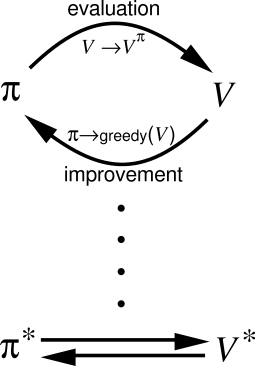
\includegraphics[width=40mm]{./graficos/gpi.png}
\caption{GPI} \label{fig:gpi}
\end{figure}


\subsection{On-policy vs Off-policy}

Los métodos on-policy tratan de evaluar y mejorar la política que está siendo usada para tomar decisiones. Imagine en cambio que queremos mejorar una determinada política $\pi$ estimando $v_\pi$ o $q_\pi$; pero sólo disponemos de episodios generados por otra política $\mu \neq \pi$. Llamamos a $\pi$ la política objetivo, porque aprender su función de valor es el objetivo del proceso de aprendizaje, mientras que a $\mu$ la llamamos política de comportamiento porque es la política que controla al agente y genera el comportamiento \cite{precup2001off}.


\subsection{Método actor-critic}

Consiste en tener una estructura de memoria separada para representar explícitamente la política independientemente de la función de valor. La estructura de la política es conocida como el actor, porque se usa para seleccionar acciones, y la función estimada de valor es conocida como el crítico, porque critica las acciones hechas por el actor \cite{barto2004j}.

Las críticas toman la forma del error, por ejemplo, en el caso de diferencias temporales, la crítica sería:

\begin{equation} \label{eq:critica_td}
\delta_t = R_{t+1} + \gamma V(S_{t+1}) - V(S_t)
\end{equation}

Donde $V$ es la función de valor actual implementada por el crítico. Este error puede ser usado para evaluar la acción recién tomada $A_t$. Si el error es positivo, la tendencia a seleccionar $A_t$ debería incrementar, pero si el error es negativo, dicha tendencia debería disminuir.


\subsection{Políticas parametrizadas}

Cuando el número de estados es demasiado grande, ya no es conveniente mantener promedios separados para cada uno en una tabla. En su lugar, el agente puede mantener la función de valor $v_\pi$ o $q_\pi$ como funciones parametrizadas y ajustar dichos parámetros para ajustarse mejor a los retornos observados. Esto también puede producir estimaciones precisas, aunque depende mucho del aproximador de función parametrizado que se escoja.


\subsection{Métodos de Gradiente de Política}

Son métodos de \ac{RL} que optimizan políticas parametrizadas respecto al retorno esperado usando la gradiente descendente \cite{sutton1999policy}.

Se asume que podemos modelar el sistema en forma de tiempo discreto y denotaremos el tiempo presente como $t$. Para tener en cuenta el factor estocástico del modelo, denotamos el cambio de estados usando una distribución de probabilidad $s_{t+1} \sim p(s_{t+1}|s_t, a_t)$ como modelo donde $a_t \in \mathbb{R}^N$ denota la acción actual, y $s_t, s_{t+1} \in \mathbb{R}^N$ denotan los estados actual y siguiente. También se asume que las acciones son generadas por una política $\pi(a_t|s_t)$ que se modela como una función de probabilidad para incorporar acciones exploratorias. Se asume que esta política está parametrizada por $k$ parámetros $\theta \in \mathbb{R}^k$. La secuencia de estados y acciones forman una trayectoria denotada por $\tau = [s_{0:H}, a_{0:H}]$ donde $H$ denota el horizonte que puede ser infinito. En cada instante de tiempo, el sistema recibe una recompensa denotada $r_t = r(s_t, a_t) \in \mathbb{R}$.

El objetivo general de la optimización de política en \ac{RL} es optimizar los parámetros de la política $\theta \in \mathbb{R}^k$ de forma que el retorno esperado se optimize.

\begin{equation}
J(\theta) = \left\lbrace \sum_{t=0}^H \gamma^t r_t \right\rbrace
\end{equation}

Para eso, los métodos de gradiente de política seguirán la gradiente ascendente del retorno esperado para actualizar los parámetros $\theta \in \mathbb{R}^k$.

\begin{equation}
\theta_{h+1} = \theta_h + \alpha_h \nabla_\theta J_{\theta = \theta_h}
\end{equation}

Donde $\alpha_h \in \mathbb{R}^+$ es la tasa de aprendizaje y $h = \{0,1,2,...\}$ es el número de la actualización actual. Nótese que el tiempo $t$ y el número de actualización $h$ son diferentes, por ejemplo, imagine un aprendizaje episódico donde la actualización se realiza sólo al final de cada episodio.


\section{Sistemas multiagente}

Un sistema multiagente es un sistema compuesto por múltiples agentes inteligentes que interactúan entre ellos. El bloque fundamental de construcción de los sistemas multiagente son los agentes, que aunque no tienen una definición formal y precisa, normalmente son vistos como entidades inteligentes, equivalentes en términos computacionales a un proceso del sistema operativo, que se pueden comunicar mediante un sistema de red.

Los agentes en un sistema multiagente tienen varias características importantes: La autonomía, visión local y descentralización, ya que no hay un agente de control designado.


\subsection{Aprendizaje en sistemas multiagente}

Sólo estudiaremos los modelos de aprendizaje con recompensa, ya que pueden ser modelados como un problema de \ac{RL}. Entre estos modelos de aprendizaje hay 4 tipos \cite{claus1998dynamics}:
\begin{itemize}
\item \textbf{Aprendizaje como un equipo}, donde los estados y las acciones incluyen a todos los agentes. De hecho se modela a todos los agentes como si fueran uno solo. Requiere de un programa centralizado que vea a todos los agentes como un todo y les indique qué hacer.
\item \textbf{Aprendizaje independiente}, donde todos los agentes conocen la ubicación de todos los agentes pero las acciones son individuales e independientes. Puede generar competición entre los agentes, llegando a un aprendizaje sub-óptimo.
\item \textbf{Aprendizaje de acciones conjuntas}, similar al aprendizaje independiente, pero involucra comunicación entre los agentes.
\item \textbf{Aprendizaje con valores de influencia}, los agentes pueden darse recompensas mutuamente para influenciar las acciones de los otros.
\end{itemize}


\section{Redes Neuronales y Deep Learning}

\subsection{Multilayer perceptron}

El \ac{MLP} es una red neuronal formada por mútliples capas que le permiten aproximar funciones no lineales \cite{yang2010multi}. La arquitectura del perceptron multicapa la podemos observar en la figura \ref{fig:mlp}.

\begin{figure}[htb]
\centering
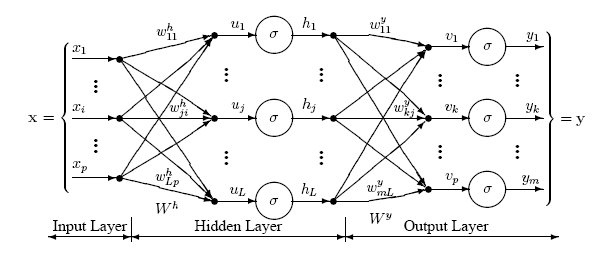
\includegraphics[width=150mm]{./graficos/mlp.jpg}
\caption{MLP} \label{fig:mlp}
\end{figure}

Básicamente tenemos entradas $x_i$ y salidas $y_i$. La red neuronal es una función paramétrica con parámetros $w$ que aproxima $y = f(x)$ modificando sus parámetros. Podemos ver a la red neuronal como una función $g(x, w) \sim f(x)$. El algoritmo que usa para aproximarse más a $f(x)$ es el de la gradiente descendente del error respecto a sus parámetros. El error puede ser cualquier función de error entre $f(x)$ y $g(x, w)$, siendo la más común la función de error cuadrático.

\begin{equation}
w = w - \alpha \nabla_w E
\end{equation}

\subsection{Restricted Boltzman Machine}

Las \ac{RBM} son redes neuronales generativas estocásticas que pueden aprender una distribución de probabilidad sobre su conjunto de entradas \cite{hinton2010practical}. La arquitectura de una \ac{RBM} se encuentra en la figura \ref{fig:rbm}. Consiste de nodos de unidades visibles $x$ y unidades escondidas $h$. Cada unidad visible está conectada a todas las unidades escondidas y viceversa. Cada conexión tiene un peso $w$ asociado, que es el parámetro que se busca optimizar mediante el entrenamiento. Cada unidad visible e invisible está desplazada por un bias $b$ o $c$. Las unidades visibles representan data observable mientras que las unidades escondidas describen las dependencias entre las variables observadas.

\begin{figure}[htb]
\centering
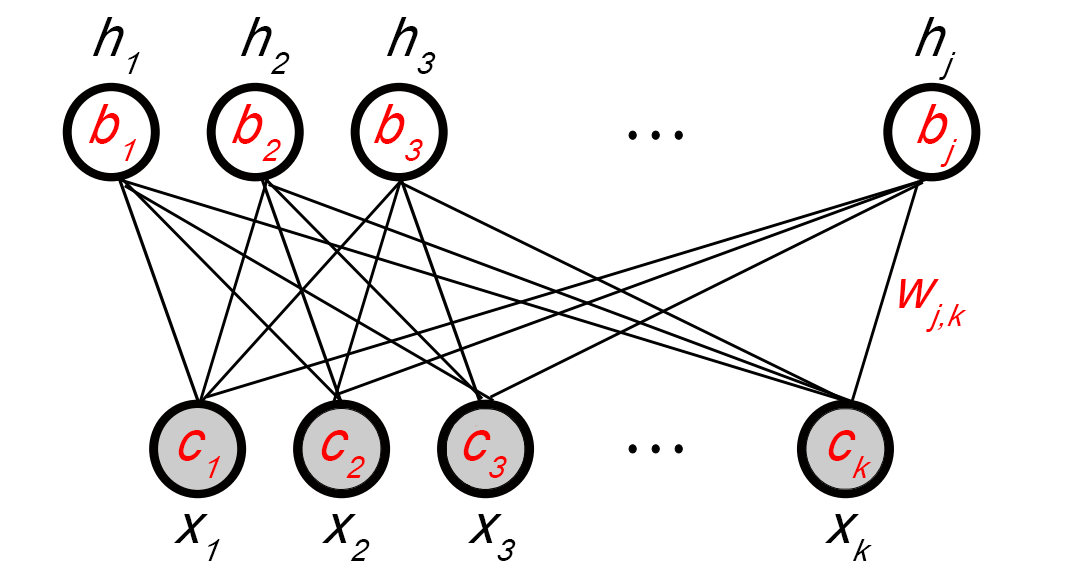
\includegraphics[width=100mm]{./graficos/rbm.png}
\caption{Arquitectura de la RBM} \label{fig:rbm}
\end{figure}

Para hallar las probabilidades se hace uso de una función de energía:

\begin{equation}
E(x, h) = -\sum_j \sum_k w_{j,k} h_j x_k - \sum_k c_k x_k - \sum_j b_j h_j
\end{equation}

El entrenamiento de esta red consiste básicamente en maximizar la probabilidad del valor de entrada. Para hacer esto se minimiza el promedio de la probabilidad logarítmica usando la gradiente descendente.


\subsection{Deep Belief Network}

En \cite{hinton2006reducing} se demostró que las \ac{RBM} podían ser apiladas y entrenadas de forma voraz para formar las llamadas Deep Belief Networks \cite{erhan2010does}. Las \ac{DBN} son modelos que aprenden a extraer una representación jerárquica profunda de los datos de entrenamiento. Modelan la distribución conjunta de un vector observado $x$ y las $l$ capas ocultas $h^k$ como sigue:

\begin{equation}
P(x, h^1, ..., h^k) = \left(\prod_{k=0}^{l-2} P(h^k|h^{k+1})\right) P(h^{l-1}, h^l)
\end{equation}

Donde $x = h^0$, $P(h^{k-1},h^k)$ es una distribución condicional para las unidades visibles condicionadas por las unidades ocultas de la \ac{RBM} en el nivel $k$, y $P(h^{l-1},h^l)$ es la distribución conjunta de las capas visible e invisible en el nivel más alto de la \ac{RBM}. Esto se ilustra en la figura \ref{fig:rbm_stack}

\begin{figure}[htb]
\centering
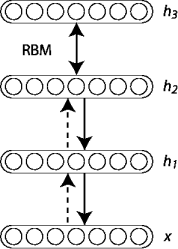
\includegraphics[width=40mm]{./graficos/rbm_stack.png}
\caption{Pila de RBM} \label{fig:rbm_stack}
\end{figure}

El principio de entrenamiento no supervisado goloso a nivel de capas puede ser aplicado a las \ac{DBN} con las \ac{RBM} como el bloque de construcción de cada capa \cite{hinton2006reducing, bengio2007greedy}. El proceso es como sigue:

\begin{enumerate}
\item Entrenar la primera capa como una \ac{RBM} que modela la entrada $x=h^0$ como su capa visible
\item Usar esta primera capa para obtener una representación de la entrada que será utilizada como data para la segunda capa. Existen dos soluciones comunes, escoger la representación como las activaciones promedio $p(h^1=1|h^0)$ o como muestras de $p(h^1|h^0)$
\item Entrenar la segunda capa como una \ac{RBM}, tomando la data transformada del paso anterior como ejemplos de entrenamiento para la capa visible de esa \ac{RBM}
\item Iterar (2 y 3) para el número deseado de capas, propagando haci arriba las muestras o activaciones promedio en cada paso
\item Ajuste fino de todos los parámetros de esta arquitectura profunda usando un criterio de aprendizaje supervisado. Por ejemplo, usando la gradiente descendente.
\end{enumerate}

\section{Consideraciones Finales}

En el siguiente capítulo veremos cómo estas ideas pueden ser usadas juntas para potenciarse mutuamente y crear un algoritmo de aprendizaje por refuerzo multiagente. Y a pesar de que surgen ciertas inconsistencias, estas son superadas con la introducción de nuevas estrategias que veremos a continuación.
